%(Aquí lo dejaría con la estructura que teníamos para Caise, presentamos el framework y posteriormente comentamos modelos y transformaciones)

In this section we present $\pi$SOD-M, an MDD based methodology.
According to MDA guidelines, $\pi$-SODM meta-models are organized into three levels: CIM (\textit{Computational Independent Models}), PIM (\textit{Platform Independent Models}) and PSM (\textit{Platform Specific Models}).

Two models are defined at the CIM level: \textit{value model}
and \textit{BPMN model}.

$\pi$SOD-M provides an environment for building service compositions.
$\pi$SOD-M includes the modelling of non-functional requirements at the early stages of the development.
The methof extends the SOD-M meta-models by adding the concept of \textit{Policy}~\cite{Espinosa-Oviedo2011a} to represent non-functional requirements.

\begin{figure}[h]
\centering
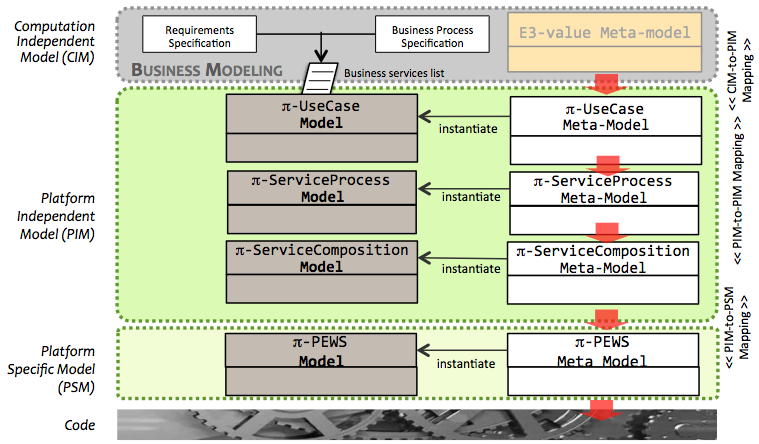
\includegraphics[width=1.0\textwidth]{figs/piSODM}
\caption{$\pi$SOD-M Overview.}
\label{fig:piSOD-M}
\end{figure}

$\pi$SOD-M (Figure~\ref{fig:piSOD-M}) proposes the generation of a set of models at different levels of abstraction, as well as transformations between these models.
$\pi$SOD-M models represent both the functional aspects of the application as well as its non-functional constraints.
Constraints are restrictions that must be verified during the execution of the application.
An example of this is the requirement of the user's authentication for executing some system functions.

Figure \ref{fig:sodm} shows  SOD-M that defines a service oriented approach   providing  a set of guidelines to build services' based information systems (SIS) \cite{decastro1,decastro2}.  Therefore, SOD-M proposes to use services as first-class objects for the whole process of the SIS  development and it  follows a Model Driven Architecture (MDA) \cite{miller}  approach. Extending from the highest level of abstraction of the MDA, SOD-M provides  a conceptual structure to: first, capture the system requirements and specification in high-level abstraction models (computation independent models, CIMÕs); next,  starting from such models build platform independent models (PIMÕs) specifying the system details; next transform such models into platform specific models (PSMÕs) that bundles the specification of the system with the details of the targeted platform; and finally, serialize such model into the working-code that implements the system. 
\begin{figure} [htpb]
\centering
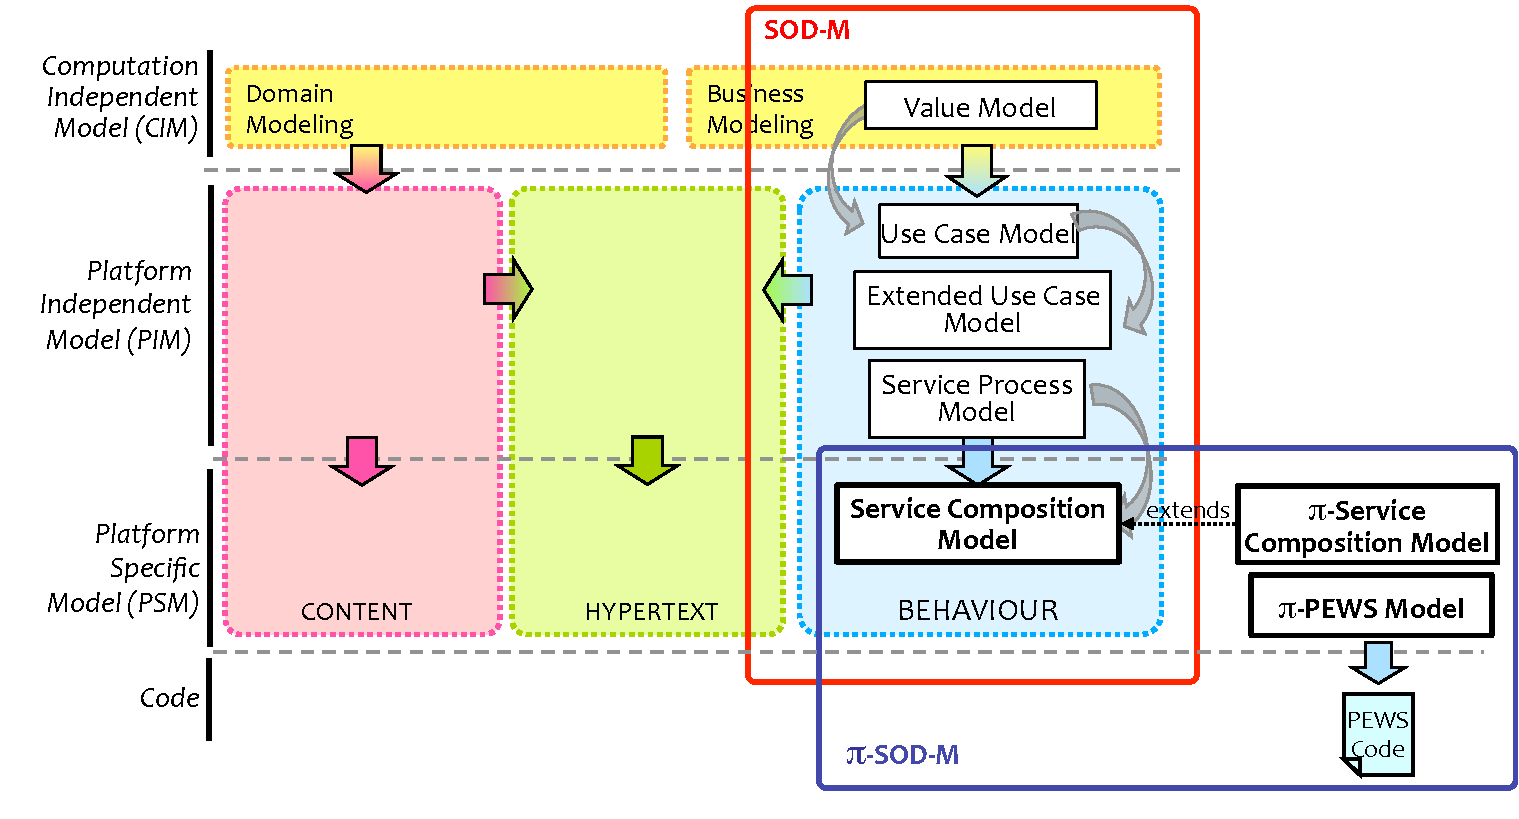
\includegraphics[width=0.65\textwidth]{figs/SODM}
\caption{SOD-M development process}
\label{fig:sodm}
\end{figure} 
As shown in Figure \ref{fig:sodm}, the SOD-M model-driven process begins by building the high-level computational independent models and enables specific models for a service platform to be obtained as a result  \cite{decastro1}. Referring to the "To Publish Music" application, using SOD-M the designer starts defining an E3value model \footnote{The E3 value model is a business model that represents a business case %graphically as a set of value exchanges ($\nabla$$\triangle$) and value activities (rounded boxes) performed by business actors (squared boxes) 
and allows  to understand the environment in which the services' composition will be placed \cite{e3value}.}  at the CIM level and then the corresponding models of the PIM are generated leading to a services' composition model (SCM).

%Similarly to SOD-M, our approach targets the construction of service-oriented applications that implement business processes.
$\pi$SOD-M proposes a development process based on the definition of models (instances of the meta-modes) and transformations between models.
There are two kinds of transformations: Model-to-model transformations are used during the software process to refine the specification.
Model-to-text transformations are the last step of the process and generate code.

%We extend SOD-M to include non-functional specifications.
Our method defines four meta-models: \textit{$\pi$-UseCase}, \textit{$\pi$-ServiceProcess}, \textit{$\pi$-ServiceCom\-po\-si\-tion} and \textit{$\pi$-PEWS}.
The former three are extensions of SOD-M meta-models and belong to the PIM level.
The \textit{$\pi$-PEWS} meta-model is a PSM.

The \textit{$\pi$-UseCase} meta-model describes functional and non-functional requirements.
Non-functional requirements are defined as \textit{constraints} over processing and data.
The \textit{$\pi$-ServiceProcess} meta-model defines the concept of \textit{service contract} to represent restrictions over data and actions that must be performed upon certain conditions.
The \textit{$\pi$-ServiceProcess} meta-model gathers the constraints
described in the \textit{$\pi$-UseCase} model into contracts that are associated
with services.
The \textit{$\pi$-ServiceComposition} meta-model provides the concept of \textit{Policy}
which put together contracts with similar non-functional requirements.
For instance, security and privacy restrictions may be grouped into a security policy.
\textit{$\pi$-ServiceComposition} models can be refined into PSMs.

At the PSM level we have lower-level models that can be automatically translated into actual computer programs.
The \textit{$\pi$-PEWS} meta-model is the PSM adopted in this work.
\textit{$\pi$-PEWS} models are textual descriptions of service compositions that can be translated into any service composition language, such as BPEL~\cite{bpel03} or PEWS~\cite{BaCAM05,Placido2010LTPD}.
This can be accomplished by defining: \textit{(i)} a model-to-model transformation, from a \textit{$\pi$-ServiceComposition} model to the corresponding PSM, and \textit{(ii)} a model-to-text transformation, from the this PSM to the composition language.



%Now, consider that besides the services' composition that represents the order in which the services are called for implementing the application "To Publish Music" it is necessary to model  other requirements that represent the (i) conditions imposed by services for being contacted, for example the fact the Facebook and Twitter require authentication protocol in order to call their methods for updating the wall; (ii) the conditions stemming from the business rules of the application logic, for example the fact that the walls in Facebook and Twitter must show the same song title and if this is not possible then none of them is updated. 
